\documentclass{article}
\usepackage{amsmath,amssymb}
\usepackage{graphicx}
\usepackage{enumerate}
\usepackage{hyperref}
\usepackage{subcaption}
\usepackage{caption}
\usepackage{xcolor}
\usepackage{float}
\hypersetup{
    colorlinks,
    linkcolor={red!50!black},
    citecolor={blue!50!black},
    urlcolor={blue!80!black}
}

\pagestyle{empty} \addtolength{\textwidth}{1.0in}
\addtolength{\textheight}{0.5in}
\addtolength{\oddsidemargin}{-0.5in}
\addtolength{\evensidemargin}{-0.5in}
\newcommand{\ruleskip}{\bigskip\hrule\bigskip}
\newcommand{\nodify}[1]{{\sc #1}}
\newcommand{\points}[1]{{\textbf{[#1 points]}}}
\newcommand{\subquestionpoints}[1]{{[#1 points]}}
\newenvironment{answer}{{\bf Answer:} \sf }{}%

\newcommand{\bitem}{\begin{list}{$\bullet$}%
{\setlength{\itemsep}{0pt}\setlength{\topsep}{0pt}%
\setlength{\rightmargin}{0pt}}}
\newcommand{\eitem}{\end{list}}

\setlength{\parindent}{0pt} \setlength{\parskip}{0.5ex}
\setlength{\unitlength}{1cm}

\newcommand{\pa}[1]{[[PA: #1]]}

\renewcommand{\Re}{{\mathbb R}}
\newcommand{\E}{{\rm E}}
\begin{document}

\pagestyle{myheadings} \markboth{}{COMP447-547 Deep Unsupervised Learning, Homework 3, Spring 2021}

{\huge
\noindent Homework 3: Latent Variable Models / GANs}
\ruleskip

{\bf Deliverable}: This PDF write-up by {\bf Wednesday April 21st, 23:59pm}.  Your PDF should be generated by simply replacing the placeholder images of this LaTeX document with the appropriate solution images that will be generated automatically when solving each question. The solution images are automatically generated and saved using the accompanying IPython notebook.  Download your results from Google Colab and replace the images in the figures/ folder with your result images. Write your name and ID in the necessary parts below, confirming the Honor Pledge. Then, you will run the .tex file to generate your PDF file. Your PDF is to be submitted into Blackboard along with your notebook, please follow the instructions given in the GitHub page. This PDF already contains a few solution images.  These images will allow you to check your own solution to ensure correctness. Note that in some parts of this report, you will need to put the final loss/accuracy values you obtained.

{\bf Honor Pledge}: ``I affirm that I have not given or received any unauthorized help on this assignment, and that this work is my own."

{\bf Name}: YOUR NAME HERE

{\bf ID}: YOUR ID HERE

\vspace{.1in}

{\bf Note}: \textit{This assignment is adapted from UC Berkeley \href{https://sites.google.com/view/berkeley-cs294-158-sp20/home}{CS294-158-SP20}}
\vspace{.2in}

%--------------------------------------------------------------------------------
%--------------------------------------------------------------------------------
%--------------------------------------------------------------------------------
\noindent {\bf Question 1: Warmup [20pt]}
%--------------------------------------------------------------------------------
%--------------------------------------------------------------------------------
%--------------------------------------------------------------------------------

\begin{enumerate}[(a)]

\item {\bf [10pt] Data from a Full Covariance Gaussian} \\\\
Final Full -ELBO: 4.4388, Recon Loss: 2.7630, KL Loss: 1.6758 (Dataset 1)
\begin{figure}[H]
    \centering
    \begin{subfigure}{0.32\textwidth}
        \centering
        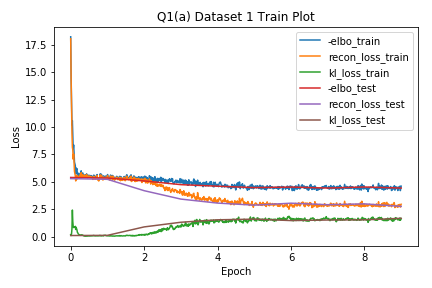
\includegraphics[width=\textwidth]{figures/q1_a_dset1_train_plot.png}
        \caption{Training curve}
    \end{subfigure}
    \begin{subfigure}{0.32\textwidth}
        \centering
        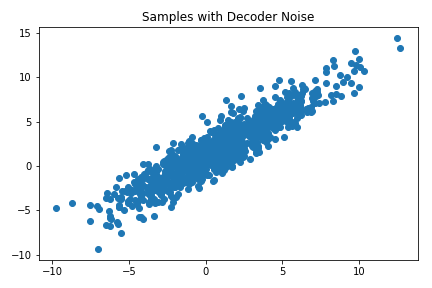
\includegraphics[width=\textwidth]{figures/q1_a_dset1_sample_with_noise.png}
        \caption{Samples with Noise}
    \end{subfigure}
    \begin{subfigure}{0.32\textwidth}
        \centering
        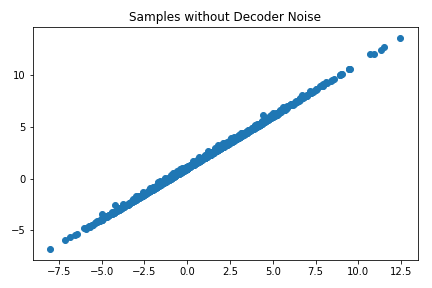
\includegraphics[width=\textwidth]{figures/q1_a_dset1_sample_without_noise.png}
        \caption{Samples without Noise}
    \end{subfigure}
    \caption{Results for Dataset 1}
\end{figure}
Final Full -ELBO: \textcolor{red}{FILL}, Recon Loss: \textcolor{red}{FILL}, KL Loss: \textcolor{red}{FILL} (Dataset 2)
\begin{figure}[H]
    \centering
    \begin{subfigure}{0.32\textwidth}
        \centering
        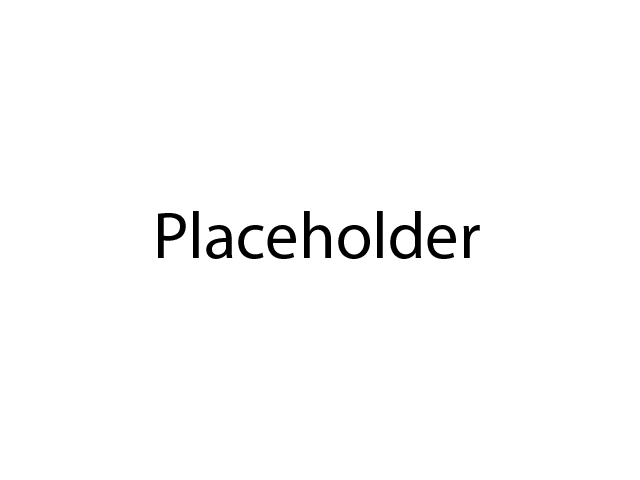
\includegraphics[width=\textwidth]{figures/q1_a_dset2_train_plot.png}
        \caption{Training curve}
    \end{subfigure}
    \begin{subfigure}{0.32\textwidth}
        \centering
        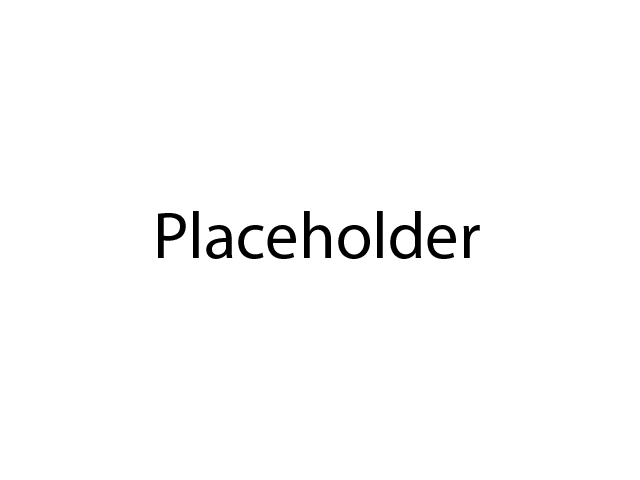
\includegraphics[width=\textwidth]{figures/q1_a_dset2_sample_with_noise.png}
        \caption{Samples with Noise}
    \end{subfigure}
    \begin{subfigure}{0.32\textwidth}
        \centering
        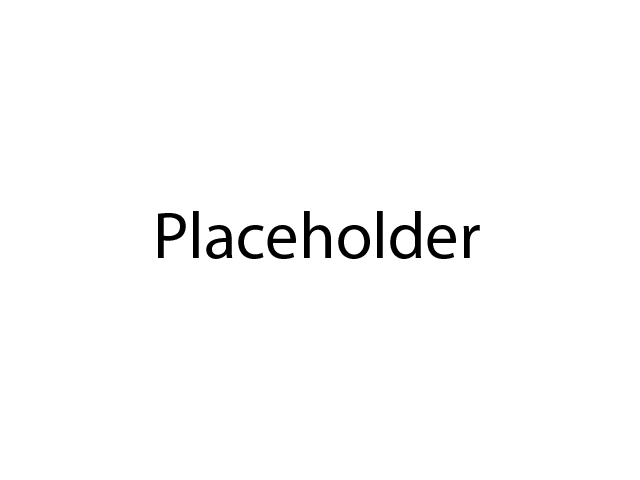
\includegraphics[width=\textwidth]{figures/q1_a_dset2_sample_without_noise.png}
        \caption{Samples without Noise}
    \end{subfigure}
    \caption{Results for Dataset 2}
\end{figure}

\newpage

\item {\bf [10pt] Minimax GAN Objective} \\\\
\begin{figure}[H]
    \centering
    \begin{subfigure}{0.45\textwidth}
        \centering
        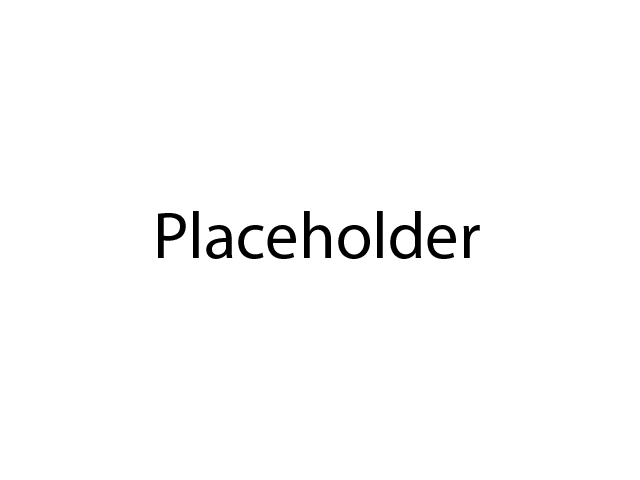
\includegraphics[width=\textwidth]{figures/q1b_epoch1.png}
        \caption{Samples at epoch 1}
    \end{subfigure}
    \begin{subfigure}{0.45\textwidth}
        \centering
        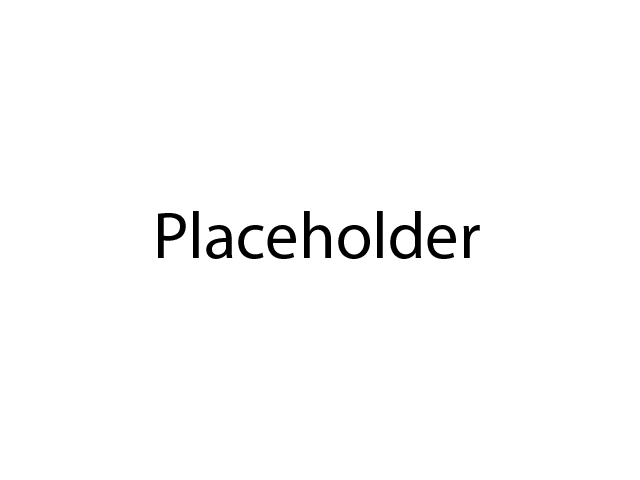
\includegraphics[width=\textwidth]{figures/q1b_final.png}
        \caption{Final samples}
    \end{subfigure}
    \\
    \begin{subfigure}{0.34\textwidth}
        \centering
        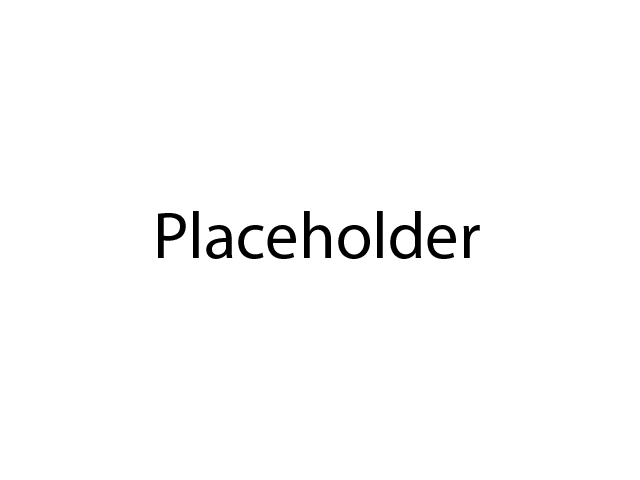
\includegraphics[width=\textwidth]{figures/q1b_losses.png}
        \caption{GAN loss curve}
    \end{subfigure}
\end{figure}
\end{enumerate}



%--------------------------------------------------------------------------------
%--------------------------------------------------------------------------------
%--------------------------------------------------------------------------------
\newpage
\noindent {\bf Question 2: VAEs on Images [40pt]}
%--------------------------------------------------------------------------------
%--------------------------------------------------------------------------------
%--------------------------------------------------------------------------------

\begin{enumerate}[(a)]
  \item {\bf [20pt] VAE} \\\\
  Final Full -ELBO: 104.0417, Recon Loss: 79.3798, KL Loss: 24.6620 (Dataset 1)
  \begin{figure}[H]
         \centering
         \begin{subfigure}[b]{0.475\textwidth}
             \centering
             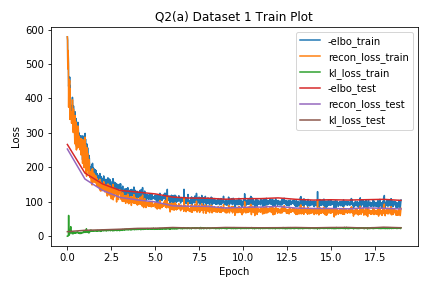
\includegraphics[width=\textwidth]{figures/q2_a_dset1_train_plot.png}
             \caption{Training Curve}
         \end{subfigure}
         \hfill
         \begin{subfigure}[b]{0.475\textwidth}
             \centering
             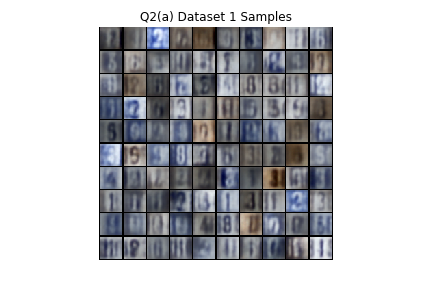
\includegraphics[width=\textwidth]{figures/q2_a_dset1_samples.png}
             \caption{Samples}
         \end{subfigure}
         \vskip\baselineskip
         \begin{subfigure}[b]{0.475\textwidth}
             \centering
             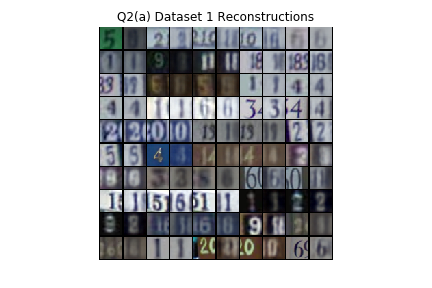
\includegraphics[width=\textwidth]{figures/q2_a_dset1_reconstructions.png}
             \caption{Reconstructions}
         \end{subfigure}
         \quad
         \begin{subfigure}[b]{0.475\textwidth}
             \centering
             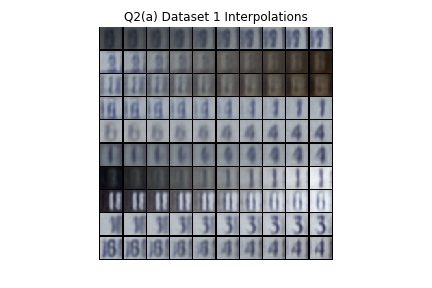
\includegraphics[width=\textwidth]{figures/q2_a_dset1_interpolations.png}
             \caption{Interpolations}
         \end{subfigure}
         \caption{Results for Dataset 1}
     \end{figure}

     \newpage

     Final Full -ELBO: \textcolor{red}{FILL}, Recon Loss: \textcolor{red}{FILL}, KL Loss: \textcolor{red}{FILL} (Dataset 2)
     \begin{figure}[H]
            \centering
            \begin{subfigure}[b]{0.475\textwidth}
                \centering
                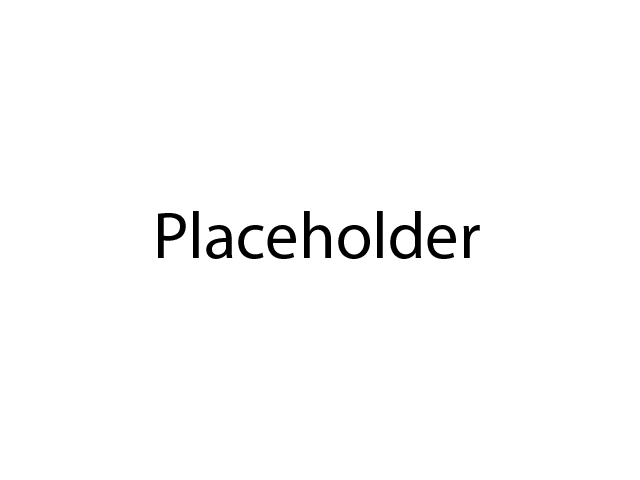
\includegraphics[width=\textwidth]{figures/q2_a_dset2_train_plot.png}
                \caption{Training Curve}
            \end{subfigure}
            \hfill
            \begin{subfigure}[b]{0.475\textwidth}
                \centering
                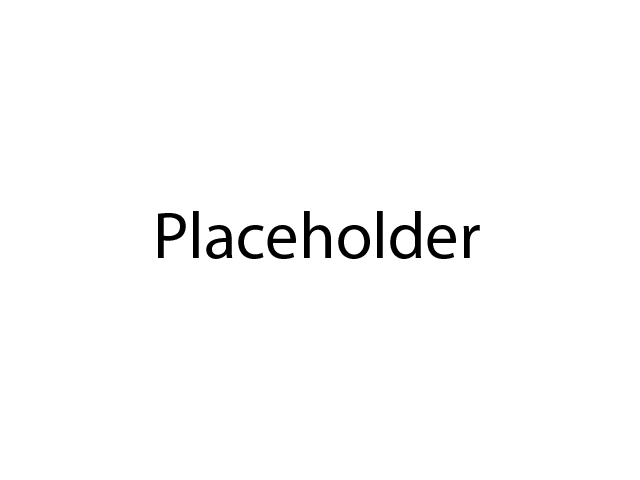
\includegraphics[width=\textwidth]{figures/q2_a_dset2_samples.png}
                \caption{Samples}
            \end{subfigure}
            \vskip\baselineskip
            \begin{subfigure}[b]{0.475\textwidth}
                \centering
                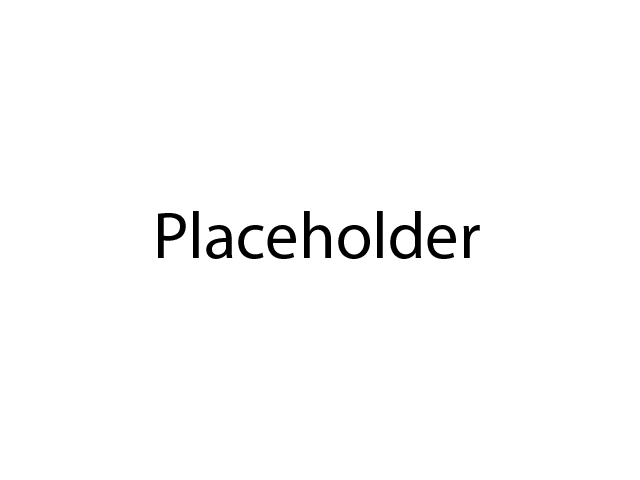
\includegraphics[width=\textwidth]{figures/q2_a_dset2_reconstructions.png}
                \caption{Reconstructions}
            \end{subfigure}
            \quad
            \begin{subfigure}[b]{0.475\textwidth}
                \centering
                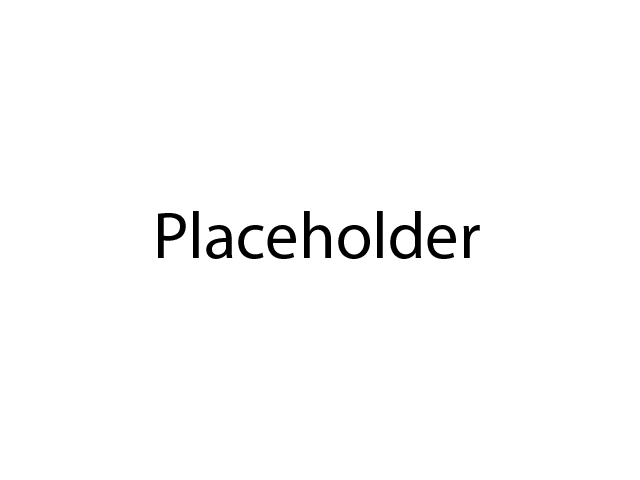
\includegraphics[width=\textwidth]{figures/q2_a_dset2_interpolations.png}
                \caption{Interpolations}
            \end{subfigure}
            \caption{Results for Dataset 2}
        \end{figure}

        \newpage

        \item {\bf [20pt] VAE with AF Prior} \\\\
        Final Full -ELBO: 102.5659, Recon Loss: 80.2548, KL Loss: 22.3111 (Dataset 1)
        \begin{figure}[H]
               \centering
               \begin{subfigure}[b]{0.475\textwidth}
                   \centering
                   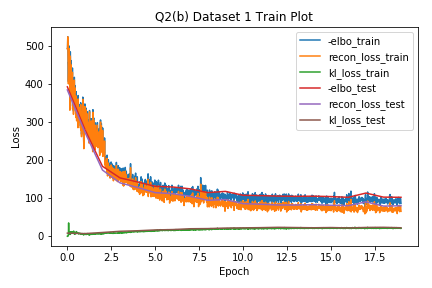
\includegraphics[width=\textwidth]{figures/q2_b_dset1_train_plot.png}
                   \caption{Training Curve}
               \end{subfigure}
               \hfill
               \begin{subfigure}[b]{0.475\textwidth}
                   \centering
                   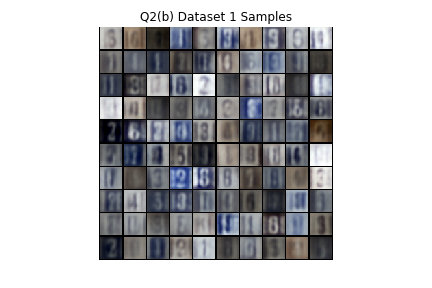
\includegraphics[width=\textwidth]{figures/q2_b_dset1_samples.png}
                   \caption{Samples}
               \end{subfigure}
               \vskip\baselineskip
               \begin{subfigure}[b]{0.475\textwidth}
                   \centering
                   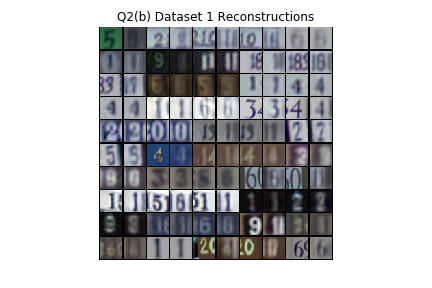
\includegraphics[width=\textwidth]{figures/q2_b_dset1_reconstructions.png}
                   \caption{Reconstructions}
               \end{subfigure}
               \quad
               \begin{subfigure}[b]{0.475\textwidth}
                   \centering
                   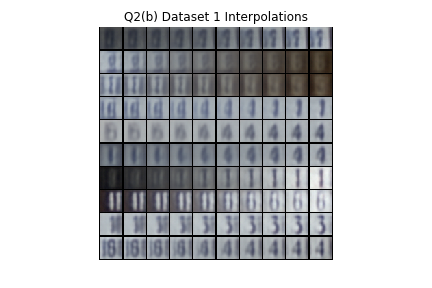
\includegraphics[width=\textwidth]{figures/q2_b_dset1_interpolations.png}
                   \caption{Interpolations}
               \end{subfigure}
               \caption{Results for Dataset 1}
           \end{figure}

           \newpage

           Final Full -ELBO: \textcolor{red}{FILL}, Recon Loss: \textcolor{red}{FILL}, KL Loss: \textcolor{red}{FILL} (Dataset 2)
           \begin{figure}[H]
                  \centering
                  \begin{subfigure}[b]{0.475\textwidth}
                      \centering
                      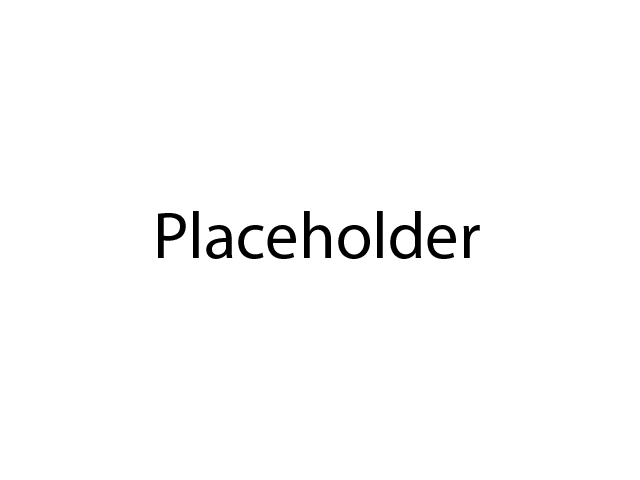
\includegraphics[width=\textwidth]{figures/q2_b_dset2_train_plot.png}
                      \caption{Training Curve}
                  \end{subfigure}
                  \hfill
                  \begin{subfigure}[b]{0.475\textwidth}
                      \centering
                      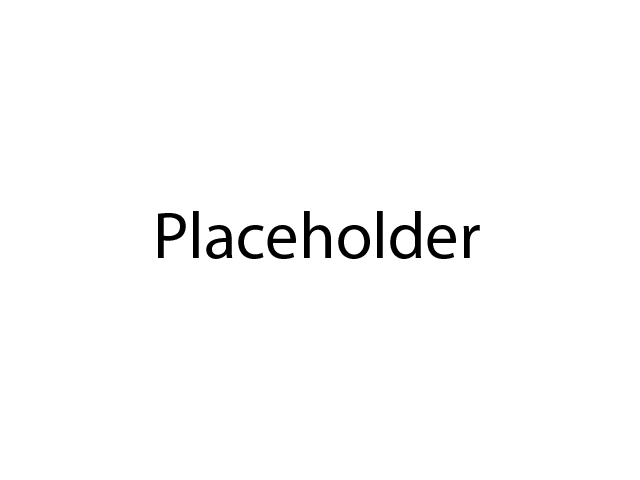
\includegraphics[width=\textwidth]{figures/q2_b_dset2_samples.png}
                      \caption{Samples}
                  \end{subfigure}
                  \vskip\baselineskip
                  \begin{subfigure}[b]{0.475\textwidth}
                      \centering
                      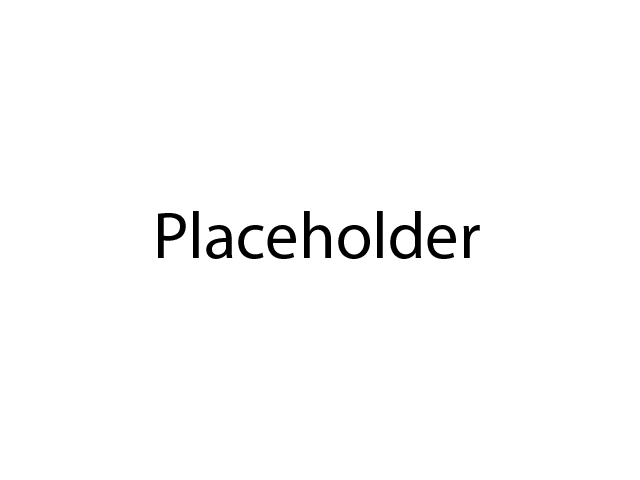
\includegraphics[width=\textwidth]{figures/q2_b_dset2_reconstructions.png}
                      \caption{Reconstructions}
                  \end{subfigure}
                  \quad
                  \begin{subfigure}[b]{0.475\textwidth}
                      \centering
                      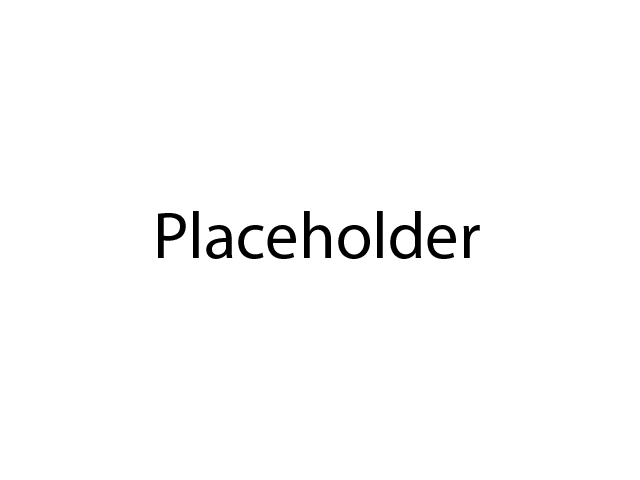
\includegraphics[width=\textwidth]{figures/q2_b_dset2_interpolations.png}
                      \caption{Interpolations}
                  \end{subfigure}
                  \caption{Results for Dataset 2}
              \end{figure}
\end{enumerate}

%--------------------------------------------------------------------------------
%--------------------------------------------------------------------------------
%--------------------------------------------------------------------------------
\newpage
\noindent {\bf Question 3: Representation Learning with BiGAN on MNIST [40 pt]}
%--------------------------------------------------------------------------------
%--------------------------------------------------------------------------------
%--------------------------------------------------------------------------------


Final BiGAN encoder test accuracy: \textbf{TODO} \\
Final random encoder test accuracy: \textbf{TODO}
\begin{figure}[H]
    \centering
    \begin{subfigure}{0.5\textwidth}
        \centering
        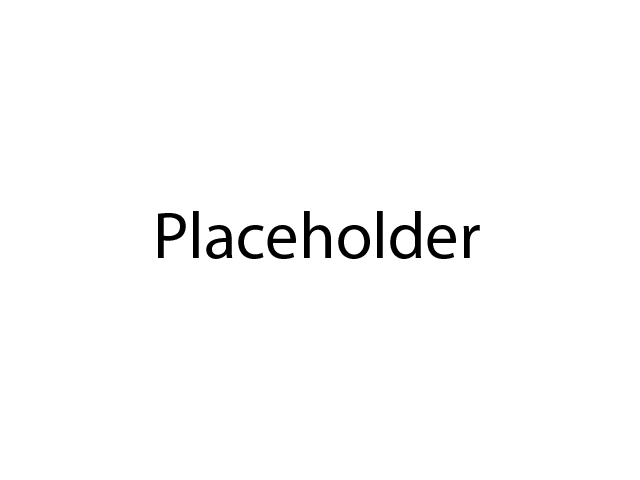
\includegraphics[width=\textwidth]{figures/q3_samples.png}
        \caption{Samples}
    \end{subfigure}
    \\
    \begin{subfigure}{0.45\textwidth}
        \centering
        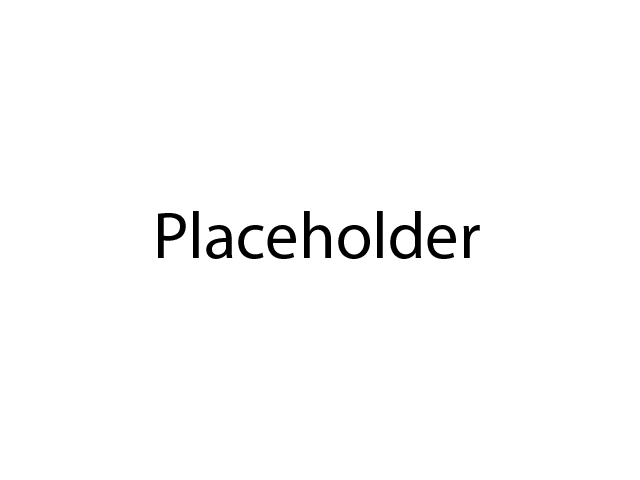
\includegraphics[width=\textwidth]{figures/q3_gan_losses.png}
        \caption{BiGAN train curve}
    \end{subfigure}
    \begin{subfigure}{0.45\textwidth}
        \centering
        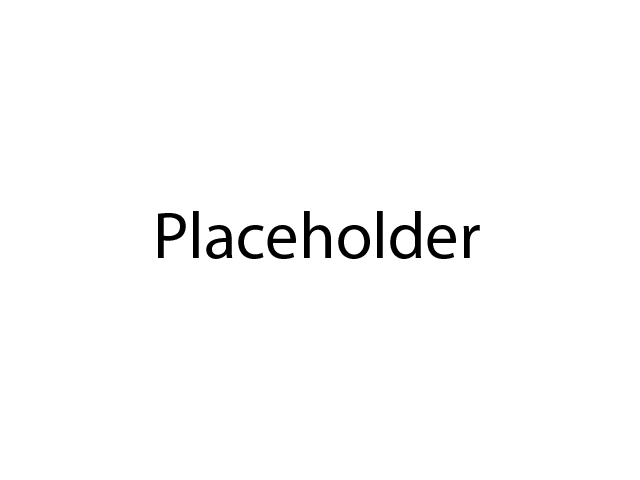
\includegraphics[width=\textwidth]{figures/q3_supervised_losses.png}
        \caption{Supervised learning curve}
    \end{subfigure}
    \\
    \begin{subfigure}{0.8\textwidth}
        \centering
        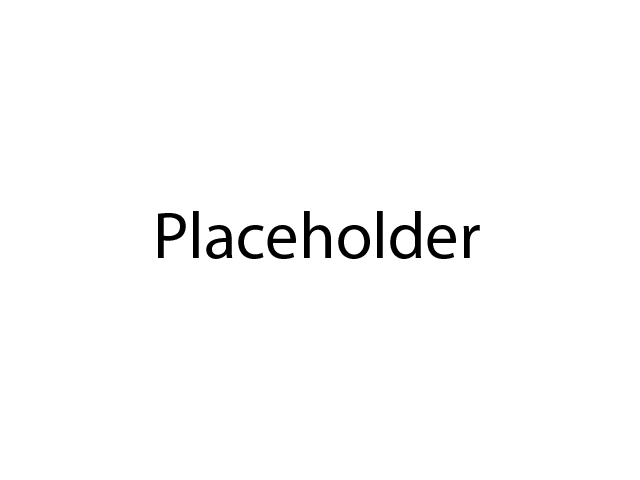
\includegraphics[width=\textwidth]{figures/q3_reconstructions.png}
        \caption{Reconstructions}
    \end{subfigure}
\end{figure}

\newpage
\noindent {\bf Bonus Questions (Optional)}
\begin{enumerate}

\item {\bf [20pt] CycleGAN} \\\\
\begin{figure}[H]
    \centering
    \begin{subfigure}{0.5\textwidth}
        \centering
        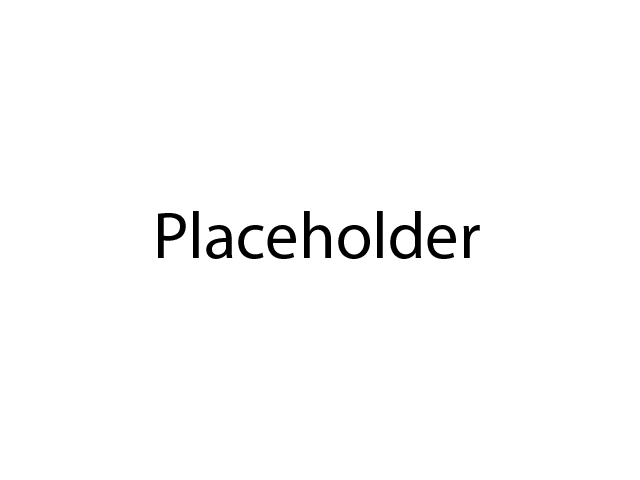
\includegraphics[width=\textwidth]{figures/q4_mnist.png}
        \caption{MNIST: original images, translations, and reconstructions}
    \end{subfigure}
    \\
    \begin{subfigure}{0.5\textwidth}
        \centering
        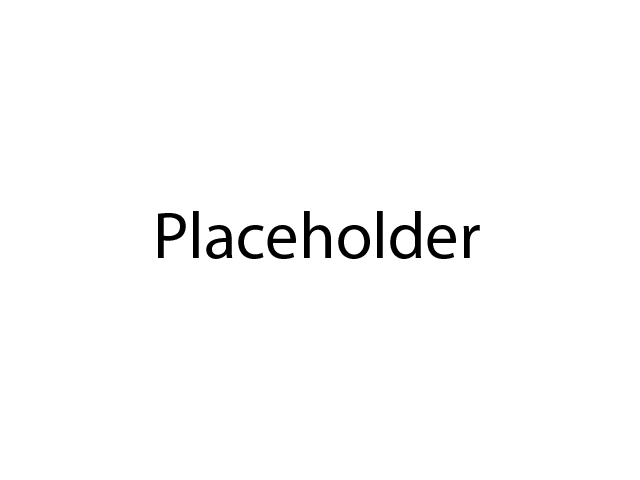
\includegraphics[width=\textwidth]{figures/q4_colored_mnist.png}
        \caption{Colored MNIST: original images, translations, and reconstructions}
    \end{subfigure}
\end{figure}
\end{enumerate}

\end{document}
